45\textwidth}
    \centering
    
\includegraphics[width=\textwidth]{wordcloud_cardioid.png} % Replace with the name of your second wordcloud image
    \caption{Cardioid-Shaped Wordcloud}
    \label{fig:wordcloud_cardioid}
  \end{minipage}
\end{figure}

\newpage

\subsection*{Network Graph Examples}

The following R code is used to create network graphs from the data:

\begin{lstlisting}[language=R]
library(igraph)
library("readxl")
data <- read_excel("C:/Users/user/Documents/data.xlsx")
x <- data.frame(data$Name, data$City)
net <- graph.data.frame(x, directed = TRUE)
V(net)
E(net)
V(net)$label <- V(net)$name
V(net)$degree <- degree(net)

hist(V(net)$degree, col = 'blue', main = 'Histogram of Node Degree', ylab = 'Frequency', xlab = 'Degree of Vertices')

set.seed(100)
plot(net, vertex.color = 'red', vertex.size = 2, edge.arrow.size = 0.5, vertex.label.cex = 0.8)
plot(net, vertex.color = rainbow(52), vertex.size = V(net)$degree * 3, edge.arrow.size = 1, layout = layout.fruchterman.reingold)
\end{lstlisting}

The following are the network graph outputs generated from the code above:

\begin{figure}[h!]
  \centering
  \begin{minipage}{0.45\textwidth}
    \centering
    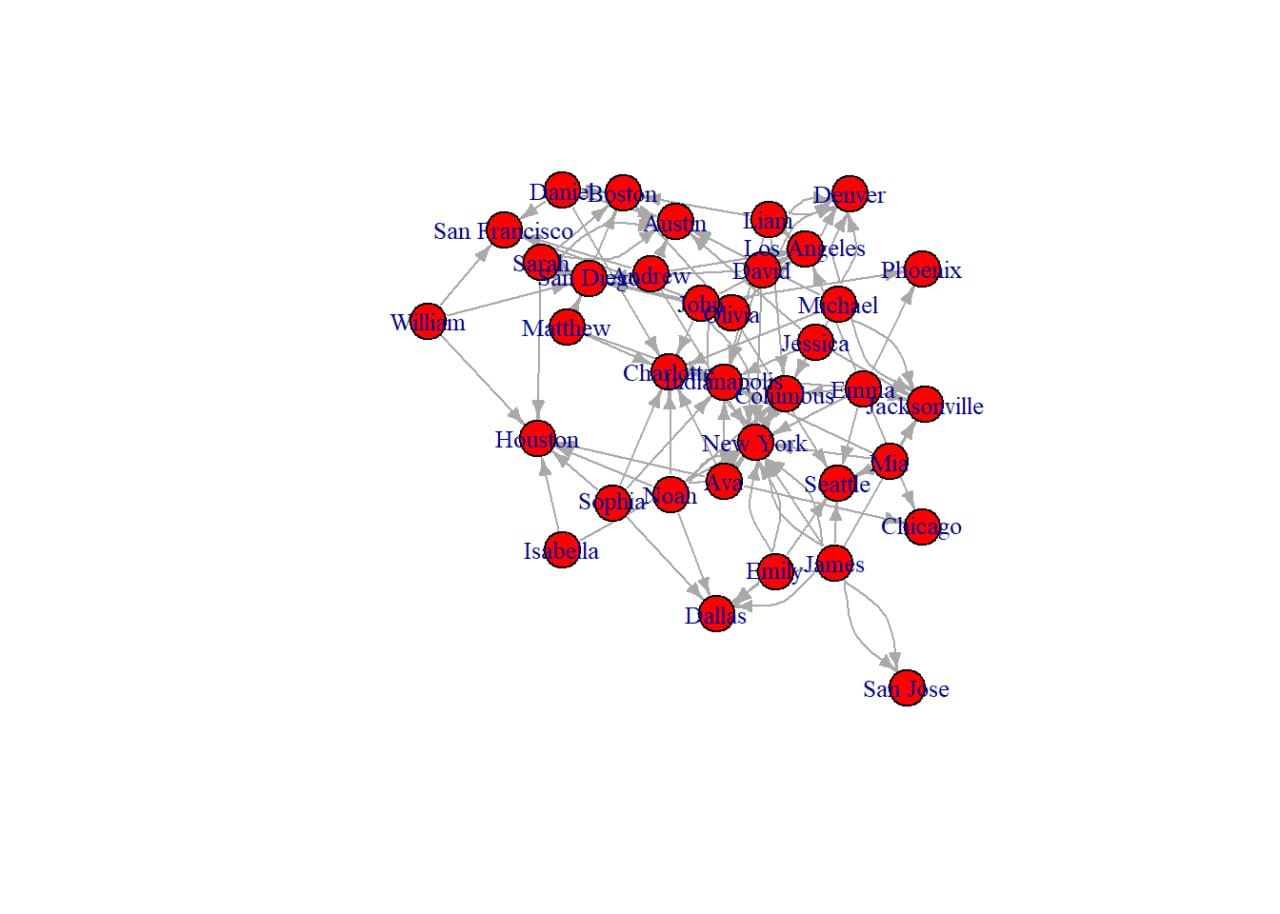
\includegraphics[width=\textwidth]{network_graph_1.png} % Replace with the name of your first network graph image
    \caption{Network Graph Example 1}
    \label{fig:networkgraph_1}
  \end{minipage} \hfill
  \begin{minipage}{0.45\textwidth}
    \centering
    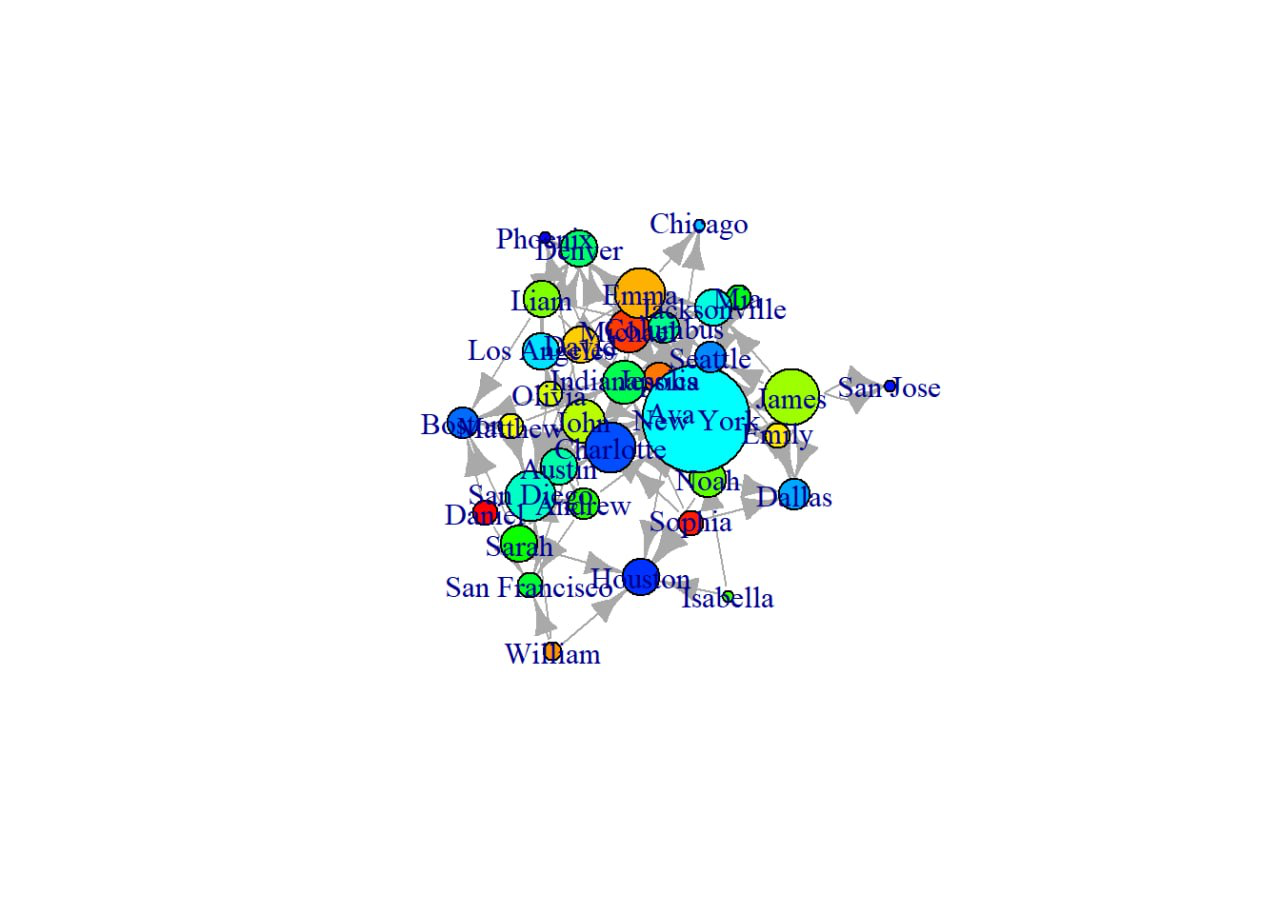
\includegraphics[width=\textwidth]{network_graph_2.png} % Replace with the name of your second network graph image
    \caption{Network Graph Example 2}
    \label{fig:networkgraph_2}
  \end{minipage}
\end{figure}

\end{document}